\section{Квадратичная форма. Положительная и отрицательная определенность. Оценка снизу положительно определенной квадратичной формы. Достаточные условия экстремума}
Сейчас нам понадобятся квадратичные формы.
Мы немного говорили о них на алгебре, но все равно вспомним основные определения и свойства.
\begin{conj}
    Функция называется квадратичная формой, если ее можно представить в виде $Q(h) = \sum\limits_{i, j = 1}^n c_{ij}h_ih_j$.
    Получается, что это некоторый многочлен второй степени от координат вектора.
\end{conj}
Тут сумма $\sum\limits_{i, j = 1}^n c_{ij}h_ih_j$ это более короткая версия $\sum\limits_{i=1}^n\sum\limits_{j=1}^n c_{ij}h_ih_j$.

Обозначим матрицу коэффициентов за $C$.
Принято считать, что она симметричная: $c_{ij} = c_{ji}$.
Мы также можем написать следующее равенство: $Q(h) = \sum\limits_{i, j = 1}^n c_{ij}h_ih_j = \langle Ch, h \rangle$.
Действительно: \begin{gather*}
    \langle Ch, h \rangle = \left \langle \begin{pmatrix}
        c_{11}h_1 + \dots + c_{1n}h_n \\
        c_{21}h_1 + \dots + c_{2n}h_n \\
        \dots \dots \\
        c_{n1}h_1 + \dots + c_{nn}h_n
    \end{pmatrix}, \begin{pmatrix}
        h_1 \\
        h_2 \\
        \dots \\
        h_n
    \end{pmatrix} \right \rangle = 
    \sum_{i=1}^n \sum_{j=1}^n c_{ij}h_jh_i
\end{gather*}

\begin{conj} Определенность квадратичной формы.

    \begin{itemize}
        \item $Q$ положительно определена, если $\forall h \in \R^n \;\; Q(h) \geqslant 0$.
        \item $Q$ отрицательно определена, если $\forall h \in \R^n \;\; Q(h) \leqslant 0$.
        \item $Q$ строго положительно определена, если $\forall h \neq 0 \in \R^n \;\; Q(h) > 0$.
        \item $Q$ строго отрицательно определена, если $\forall h \neq 0 \in \R^n \;\; Q(h) < 0$. 
    \end{itemize}
\end{conj}

\vspace*{5mm}

\begin{lemma}
    Если $Q(h)$ строго положительно определена, то $\exists c > 0$, т.ч. $Q(h) \geqslant c\|h\|^2 $
\end{lemma}
\begin{proof}
    Заметим, что $Q(h) = \langle Ch, h \rangle$ -- непрерывная функция.
    Давайте рассмотрим ее на единичной сфере (обобщение единичной окружности).
    Это компактное множество, а мы знаем, что непрерывная функция на компакте обязана принимать свое минимальное значение: $\exists h_0 : \|h_0\| = 1$ и $Q(h) \geqslant Q(h_0) \;\; \forall h : \|h\| = 1$.
    
    Положим $c = Q(h_0)$ и докажем, что оно подходит.
    Все, что нам надо сделать, это просто отнормировать вектор и воспользоваться неравенством: \[ \forall h \;\; Q(h) = \langle Ch, h \rangle = \|h\|^2 \left\langle C \frac{h}{\|h\|}, \frac{h}{\|h\|} \right\rangle = \|h\|^2Q\left(\frac{h}{\|h\|}\right) \geqslant c\|h\| \]
\end{proof}

\begin{theorem} [достаточные условия экстремума]
    Пусть $f: E \to \R$, $a$ -- стационарная точка, $f$ дважды дифференцируема в точке $a$, $Q(h) = \sum\limits_{i, j = 1}^n f''_{x_ix_j}(a)h_ih_j$ -- квадратичная форма. Тогда: \begin{enumerate}
        \item Если $Q$ строго положительно (отрицательно) определена, то $a$ -- строгий локальный минимум (максимум).
        \item Если $a$ -- нестрогий локальный минимум (максимум), то $Q$ нестрого положительно (отрицательно) определена.
    \end{enumerate}
\end{theorem}
\begin{proof} \quad
    \begin{enumerate}
        \item Будем доказывать для минимума.
        Воспользуемся формулой Тейлора для стационарной точки: \begin{gather*}
            f(a + h) = f(a) + \frac{1}{2} \sum_{i, j = 1}^n f''_{x_ix_j}(a)h_ih_j + o(\|h\|^2) \\
            \Rightarrow f(a + h) - f(a) = \frac{1}{2}Q(h) + o(\|h\|^2) = \frac{1}{2}Q(h) + \alpha(h)\|h\|^2, \text{ где } \alpha(h) \to 0 \text{ при } h \to 0
        \end{gather*}
        Воспользуемся леммой: \[ f(a+h) - f(a) =  \frac{1}{2}Q(h) + \alpha(h)\|h\|^2 \geqslant \frac{c}{2}\|h\|^2 + \alpha(h)\|h\|^2 = \|h\|^2 \left(\frac{c}{2} - \alpha(h) \right)  \]
        Осталось заметить, что при малых $h$ множитель $(\frac{c}{2} - \alpha(h)) > 0$, следовательно, $f(a + h) - f(a) > 0$, а это означает, что $a$ -- строгий локальный минимум.
        \item Опять же будем доказывать только для минимума. 
        Зафиксируем произвольное $h$.
        Мы хотим показать, что $Q(h) \geqslant 0$. 
        Воспользуемся все той же формулой Тейлора, но только теперь, так как $h$ фиксировано, введем вспомогательный параметр $t$:
        \[ f(a + th) - f(a) = \frac{1}{2}Q(th) + \underbrace{o(t^2\|h\|^2)}_{= o(t^2)} \]
        Вынесем $t$ из под квадратичной формы (в каждом слагаемом у нас есть умножение на $t^2$): 
        \begin{gather*}
            f(a + th) - f(a) = t^2 \left(\frac{Q(h)}{2} + o(1) \right) \\
            \frac{f(a + th) - f(a)}{t^2} = \frac{Q(h)}{2} + o(1)
        \end{gather*}
        Вследствие того, что $a$ -- локальный минимум, выражение $\frac{f(a + th) - f(a)}{t^2} \geqslant 0$.
        Устремим $t$ к нулю, чтобы убрать $o(1)$, и получим, что $\frac{Q(h)}{2} \geqslant 0$.
    \end{enumerate}
\end{proof}

\notice \, Если $Q$ не имеет нестрогую знакоопределенность (то есть меняет знак), то $a$ не точка экстремума.

\vspace*{5mm}

\textit{Дальше идет дополнительная информация, формально, она не относится к билету.}

А как по матрице квадратичной формы понять, что она положительно определена? Или строго положительно?
На этот вопрос помогает ответить критерий Сильвестра, который мы оставим без доказательства.

\textbf{Критерий Сильвестра.} Путь $Q(h) = \langle Ch, h \rangle$. 
Тогда чтобы понять определенность $Q$, надо посмотреть на последовательность знаков определителей следующих миноров: \begin{gather*}
    \begin{vmatrix}
        c_{11}
    \end{vmatrix}, \begin{vmatrix}
        c_{11} & c_{12} \\
        c_{21} & c_{22}
    \end{vmatrix}, \begin{vmatrix}
        c_{11} & c_{12} & c_{13} \\
        c_{21} & c_{22} & c_{23} \\
        c_{31} & c_{32} & c_{33}    
    \end{vmatrix}, \dots, \begin{vmatrix}
        c_{11} & \dots & c_{1n} \\
        \dots & \dots & \dots \\
        c_{n1} & \dots & c_{nn} 
    \end{vmatrix}
\end{gather*} 
\begin{itemize}
    \item Если они все $> 0$, то форма строго положительно определена.
    \item Если они все $\geqslant 0$, то форма положительно определена.
    \item Если они образуют знакочередующуюся последовательность, начинающуюся с отрицательного числа, то мы можем говорить про (строгую, если все знаки строгие) отрицательную определенность.
\end{itemize}

\begin{example}
    Найдем экстремумы у функции $f(x, y) = x^4 + y^4 - 36xy$.

    Для начала надо найти стационарные точки.
    Функция везде дифференцируемая, так что надо просто найти точки, в которых градиент равен 0: \begin{gather*}
        \begin{cases}
            f'_x(x, y) = 4x^3 - 36y = 0 \\
            f'_y(x, y) = 4y^3 - 36x = 0
        \end{cases}
    \end{gather*}
    Несложно проверить, что это будут точки $\{ (3, 3), (-3, -3), (0, 0) \}$.
    Чтобы посчитать нужную квадратичную форму, нам нужны вторые производные: \begin{gather*} 
        f''_{xx}(x, y) = 12x^2 \quad f''_{yy}(x, y) = 12y^2 \quad f''_{xy}(x, y) = f''_{yx}(x, y) = -36 \\
        \Rightarrow Q(x, y) = \begin{pmatrix}
            12x^2 & -36 \\
            -36 & 12y^2
        \end{pmatrix}
    \end{gather*}
    Осталось подставить конкретные точки и по критерию Сильвестра определить, какая у нас форма: \begin{itemize}
        \item Для точки $(3, 3)$ последовательность определителей выглядит как $\{ 9, 72 \}$, значит форма строго положительно определена, и $(3, 3)$ -- строгий минимум.
        \item Для точки $(-3, -3)$ все аналогично.
        \item Для точки $(0, 0)$ получаем последовательность $\{ 0, -9 \}$, значит, форма не имеет нестрогую знакоопределенность, и $(0, 0)$ не точка экстремума.
    \end{itemize}
\end{example} 

\vspace*{5mm}

Почему не все точки, у которых частные производные 0, являются экстремумами?
Может так оказаться, что по одним координатам точка является локальным минимумом, а по другим -- локальным максимумом.
Такие точки называются седловыми. 
Ниже представлен пример для $f(x, y) = x^2 - y^2$.

\begin{center}
    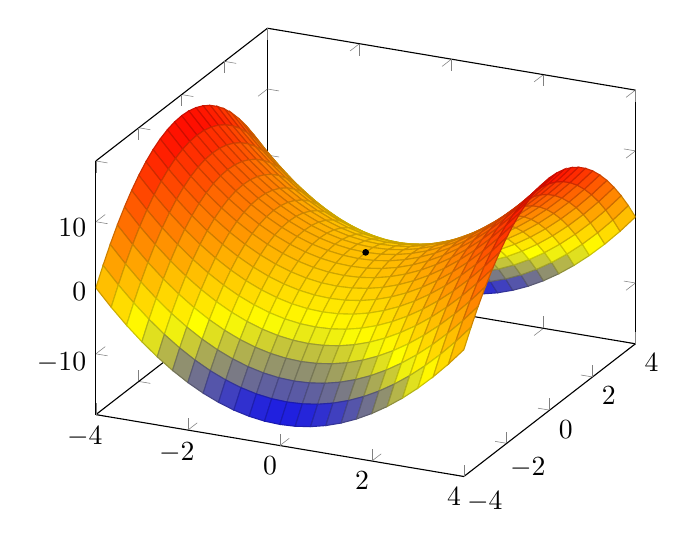
\begin{tikzpicture}
        \begin{axis}
            \addplot3 [
                surf,
                shader=faceted,
                samples=25,
                domain=-4:4,
                y domain=-4:4
                ] {x^2-y^2};
            \filldraw[black] (axis cs:0,0,0) circle(1pt);
        \end{axis}
    \end{tikzpicture}
\end{center}